\documentclass{article}

% if you need to pass options to natbib, use, e.g.:
%     \PassOptionsToPackage{numbers, compress}{natbib}
% before loading neurips_2021

% ready for submission

% to compile a preprint version, e.g., for submission to arXiv, add add the
% [preprint] option:
%     \usepackage[preprint]{neurips_2021}

% to compile a camera-ready version, add the [final] option, e.g.:
\usepackage[final]{workshop}

% to avoid loading the natbib package, add option nonatbib:
%    \usepackage[nonatbib]{neurips_2021}

\usepackage{wrapfig}
\usepackage{graphicx}
\usepackage{fontawesome}

\usepackage[utf8]{inputenc} % allow utf-8 input
\usepackage[T1]{fontenc}    % use 8-bit T1 fonts
\usepackage{hyperref}       % hyperlinks
\usepackage{url}            % simple URL typesetting
\usepackage{booktabs}       % professional-quality tables
\usepackage{amsfonts}       % blackboard math symbols
\usepackage{nicefrac}       % compact symbols for 1/2, etc.
\usepackage{microtype}      % microtypography
\usepackage{xcolor}         % colors

\usepackage{float}
\usepackage{pgf}
\usepackage{tikz}
\usetikzlibrary{arrows,automata,snakes}
\usepackage{rotating}

\usepackage{abstract}
\renewcommand{\abstractname}{}    % clear the title
\renewcommand{\absnamepos}{empty} % originally center


\title{Advances in Programming Languages\\ and Neurosymbolic Systems (AIPLANS)}

% The \author macro works with any number of authors. There are two commands
% used to separate the names and addresses of multiple authors: \And and \AND.
%
% Using \And between authors leaves it to LaTeX to determine where to break the
% lines. Using \AND forces a line break at that point. So, if LaTeX puts 3 of 4
% authors names on the first line, and the last on the second line, try using
% \AND instead of \And before the third author name.

\author{%
    Breandan Considine$^{1, 4}$, Disha Shrivastava$^{1, 3, 4}$, David Yu-Tung Hui$^{2, 4}$ \\
    \textbf{Chin-Wei Huang$^{2, 4}$, Shawn Tan$^{2, 4}$, Xujie Si$^{1, 4}$, Prakash Panangaden$^{1, 4}$} \\
    McGill University$^1$, Universit\'e de Montr\'eal$^2$, Google Research$^3$, Mila$^4$ \\
    \texttt{\{considib, shrivast, huidavid, huangchi, tanjings,}\\
    \texttt{xujie.si, prakash.panangaden\}@mila.quebec} \\
}

\begin{document}

    \maketitle
    \vspace{-0.5cm}
    \begin{abstract}
        % A very brief advertisement or tagline for the workshop, up to 140 characters, that highlights any key information you wish prospective attendees to know, and which would be suitable to be put onto a web-based survey (see below).
        \textbf{Tagline:} AIPLANS: a new workshop at NeurIPS 2021 fusing ML with programming theory to create neurosymbolic program-writing machines!  \url{https://aiplans.github.io} % Are you curious whether machines can write programs that are both sound and interpretable? Come check out AIPLANS, a new workshop on domain-specific languages for learning and synthetic reasoning, to be hosted at NeurIPS 2021!
    \end{abstract}


    % A title and a brief description of the workshop topic and content.
    Neural information processing systems have benefited tremendously from the availability of programming languages and frameworks for automatic differentiation (AD). Not only do NeurIPS benefit from \textbf{programming languages} for automatic inference but can also be considered as a language in their own right, consisting of differentiable and stochastic primitives. Combined with neural language models, these systems are increasingly capable of generating symbolic programs a human programmer might write in a high-level language. Developing \textbf{neurosymbolic systems} for automatic program synthesis requires insights from both statistical learning and programming languages.

    AIPLANS invites all researchers working towards the same purpose in these two communities to build on common ground. Our workshop is designed to be as inclusive as possible towards researchers engaged in building programming languages and neurosymbolic systems of various forms:
    \begin{itemize}
        \item \textbf{Machine learning researchers} would present advances in meta-learning, reinforcement learning and program synthesis. AIPLANS would afford these participants an opportunity to learn about new automatic programming languages and techniques for inference.
        \item \textbf{Language designers} would be able to give tutorials on newly developed software such as JAX, DEX, PyTorch and their latest features. AIPLANS would give them an opportunity to engage their users and stay in touch with the community's needs and research directions.
        \item \textbf{PL theorists} would present fundamental theory behind the design of automatic programming languages, such as functional, semiring or array programming. At AIPLANS, they would gain a better understanding of practical research problems the ML community is tackling.
        \item \textbf{Probabilistic programming researchers} would present advances in, e.g., Bayesian program synthesis and neurosymbolic systems. AIPLANS would provide a opportunity for them to understand how their work bridges the divide between PL theory and practice.
    \end{itemize}

    % These three paragraphs are not that important.  If low on space, delete
    %%%%%%%%%%%%%%%%%%%%%%%%%%%%%%%%%%%%%%%%%%%%%%
    While other workshops have explored these themes separately, few have highlighted the synergies between them. As these fields have traditionally been segregated, rediscovery of ideas was common. AD itself was invented a half dozen times over the last century and research continues to reveal unexpected connections to implicit differentiation, bilevel optimization, optimal control, stochastic processes and differential equations.  Semiring programming has existed for many decades and shares deep connections to reinforcement learning, structured inference and probabilistic programming.

    Likewise, many recently-transplanted ideas in machine learning are catechism in the programming language literature.  For example, functional and type-safe programming are lingua franca in PL circles but relatively new to Python, the primary language used in machine learning.  The duality between code and data is well-known in PL under the aegis of homoiconicity. PL theory has thought carefully about categorical semantics, process calculi, linear logic, type theory and other deeply useful concepts which remain, to this day, largely unfamiliar to the machine learning community.

    % In contrast, PL has long wrestled with the distinction between intensional and extensional representation, a distinction which the statistical learning community has long since reconciled through model-based learning and approximation theory.
    \pagebreak
    Other areas where the interaction could be fruitful are tools for equivalence, proof search and metrics. A deeper understanding of programming language semantics are largely missing from neural program synthesis discussions. The connection between various forms of message passing in concurrent systems and neural science merits further investigation. New language models could enable more effective tools for natural language and assistive programming. While some of these topics remain greenfield research topics, many connections are known, but yet-to-be-translated textbook knowledge.

    \begin{figure}[H]
        \centering
        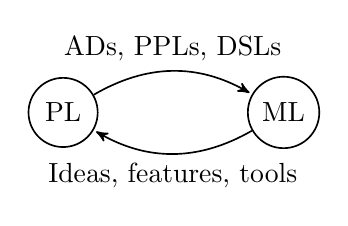
\begin{tikzpicture}[->,>=stealth',shorten >=1pt,auto,node distance=2.8cm, semithick]
            % \tikzstyle{every state}=[draw=none,text=white]

            \node[state]         (A)                    {PL};
            \node[state]         (B) [right of=A]       {ML};

            \path (A) edge [bend left] node {ADs, PPLs, DSLs} (B)
            (B) edge [bend left] node {Ideas, features, tools} (A);
        \end{tikzpicture}
        \caption{The virtuous cycle of machine learning and programming languages research.}
    \end{figure}

    Applying techniques from programmable inference to transform and generate programs, and adapting insights gained developing those programs to drive innovation in higher-order AD and probabilistic programming is a virtuous cycle. As researchers grow more accustomed to outsourcing low-level reasoning tasks to automatic programming systems, we anticipate cooperation between automatic and synthetic programming will continue to increase.  A joint workshop such as the one put forward in this proposal could help to facilitate yet-unrealized research connections among neighboring fields.
    %%%%%%%%%%%%%%%%%%%%%%%%%%%%%%%%%%%%%%%%%%%%%%%%%%


    % Much work remains.
    % Similar domain-specific languages have shown progress automating inference in other logical disciplines, such as belief nets, proof nets, and related message passing schemes on tree- and graph-structured data.

    % For example, functional and type-safe programming are lingua franca in PL circles but relatively new to Python, the primary language used in machine learning. PL theory has thought deeply about categorical semantics, concurrency, process calculi, linear logic, privacy and other deeply useful concepts which remain, to this day, mostly unfamiliar in the machine learning community.  Similarly, the programming language community too, has its blind spots. PL could take a page from structured inference and propagation algorithms as a medium for distributed computation.

    % In exchange, we believe a great deal of progress can be achieved, in particular, between automatic and synthetic programming. For illustration, we include the following incomplete list of topics:

    % \begin{itemize}
    % \item Differentiable programming / algorithmic differentiation
    % \item Probabilistic programming / statistical inference
    % \item Dynamic programming / reinforcement learning
    % \item Program induction / program synthesis
    % \item Functional programming / $\lambda$-calculus
    % \item Semiring programming / message passing
    % \item Array programming / linear algebra
    % \item Meta-programming / meta-learning
    % \item Logic programming / Relational programming
    % \end{itemize}



    % A description of special requirements and technical needs.
    % TODO




    % A list of invited speakers, if applicable, with an indication of which ones have already agreed and which are indicative.
    % We plan to invite four keynote speakers.  Three system developers, and one programming language theoretician.  TODO:
    % \begin{itemize}
    %     \item
    % \end{itemize}







    % An account of the efforts made to ensure diversity of the organizers and speakers (WiML, Black in AI, and LXAI directories, among others, may be a useful resource). Also an account of any efforts to include diverse participants (e.g., via mentoring, subsidies, or the wording and topics in the CFP).
    AIPLANS will be a single-day workshop hosted online, enabling an economically and geographically diverse audience to participate. Talks will be hosted in English, following the standard format of oral presentations and panel discussions, to be concluded with a virtual poster session. Proceedings will be non-archival. Outside of standard videoconferencing and SlidesLive assistance, we anticipate no other technical requirements. If accepted, we expect to receive a hundred or so participants, including speakers and workshop submitters, based on attendance at similarly-themed workshops in prior years.
    % An estimate of the number of attendees.

    Those who traditionally publish in venues such as SIGPLAN and SIGSOFT are encouraged to submit work that may be relevant to the machine learning and reasoning community, provided that effort is taken to ensure its accessibility. Special consideration will be given to didactic submissions of outstanding clarity. Further information, including evaluation criteria, examples of relevant literature, deadlines and workshop logistics will be made available in a timely manner.

    %   By submitting a workshop proposal, workshop organizers commit to notifying those who submit contributions (including talks and posters) to the workshop of their acceptance status before Oct 22, 2021. A timeline should be included in the proposal that will allow for this.

    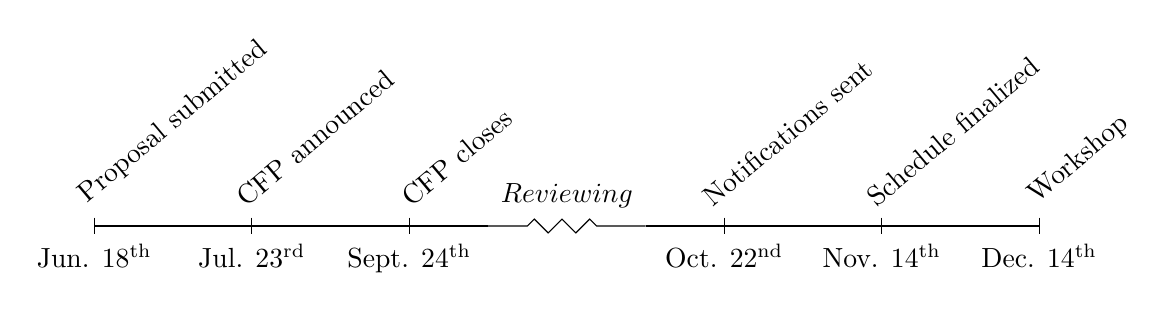
\begin{tikzpicture}[snake=zigzag, line before snake = 5mm, line after snake = 5mm]
        % draw horizontal line
        \draw (0,0) -- (5,0);
        \draw[snake] (5,0) -- (7,0);
        \draw (7,0) -- (12,0);


        % draw vertical lines
        \foreach \x in {0, 2, 4, 8, 10, 12}
        \draw (\x cm,3pt) -- (\x cm,-3pt);

        % draw nodes

        \draw (0,0) node[below=3pt] {Jun. 18\textsuperscript{th}} node[above=3pt] {};
        \draw (1,0) node[below=3pt] {} node[above=3pt] {$\begin{turn}{40}  Proposal submitted \end{turn} $};
        \draw (2,0) node[below=3pt] {Jul. 23\textsuperscript{rd}} node[above=3pt] {};

        \draw (2.8,0) node[below=3pt] {} node[above=3pt] {$\begin{turn}{40}  CFP announced \end{turn} $};
        \draw (4,0) node[below=3pt] {Sept. 24\textsuperscript{th}} node[above=3pt] {};
        \draw (4.6,0) node[below=3pt] {} node[above=3pt] {$\begin{turn}{40}  CFP closes \end{turn} $};
        \draw (6,0) node[below=3pt] {} node[above=3pt] {$ Reviewing $};
        \draw (8,0) node[below=3pt] {Oct. 22\textsuperscript{nd}} node[above=3pt] {};
        \draw (8.8,0) node[below=3pt] {} node[above=3pt] {$\begin{turn}{40}  Notifications sent \end{turn} $};
        \draw (10,0) node[below=3pt] {Nov. 14\textsuperscript{th}} node[above=3pt] {};
        \draw (10.9,0) node[below=3pt] {} node[above=3pt] {$\begin{turn}{40}  Schedule finalized \end{turn} $};
        \draw (12,0) node[below=3pt] {Dec. 14\textsuperscript{th}} node[above=3pt] {};
        \draw (12.5,0) node[below=3pt] {} node[above=3pt] {$\begin{turn}{40} Workshop \end{turn} $};
    \end{tikzpicture}

    If accepted, AIPLANS will announce its CFP and pursue contributions from the broader ML/PL community shortly thereafter. Two months later, the CFP will close on Sept. 24\textsuperscript{th}. This deadline may be extended to no later than Oct. 1\textsuperscript{st}, depending on the volume of submissions received, leaving sufficient time for referees and program chairs to leave feedback. Authors will be notified of acceptance no later than Oct. 22\textsuperscript{nd}. We intend to finalize the schedule and coordinate presentation logistics between Nov. and Dec. 14\textsuperscript{th}. Those who wish to prerecord talks will be given an opportunity to do so. The final workshop will consist of prerecorded and live talks with Q\&A, followed by a moderated panel, and virtual poster session hosted on GatherTown. Further details about schedule and logistics will be made available, pending acceptance at: \url{https://aiplans.github.io/}.

    AIPLANS is an equal-opportunity workshop that celebrates cultural, linguistic, ethnic and intellectual diversity in all forms. Not only are we committed to nondiscrimination on the basis of, e.g., race, creed, age, gender, orientation, physical or mental handicap, but also aim to encourage individuals from other disadvantaged and underrepresented socioeconomic backgrounds to participate. Should our workshop be accepted, scholarships covering the cost of registration will be extended for those who wish to attend but would otherwise be unable to do so due to financial hardship.


    \newpage


    \section*{Organizers}\vspace{-0.5cm}
    \begin{figure}[H]
        \begin{wrapfigure}{l}{0.2\textwidth}
            
\includegraphics[width=0.2\textwidth]{organizers/breandan}
        \end{wrapfigure}
        \textbf{Breandan Considine} is a Ph.D. student at McGill University supervised by Jin Guo. His research studies the relationship between software and machine learning, reasoning about the behavior of real-world programs and using those insights to build more intelligent programming tools for developers. This year, he co-organized the ICLR workshop, \href{https://rethinkingmlpapers.github.io/}{Rethinking ML Papers}. Previously, Breandan obtained his Master's degree from the Universit\'e de Montr\'eal, where he studied differentiable programming and software engineering. He is enthusiastic about AI as a tool for augmenting human reasoning and eager to help bring together the programming language and machine learning communities.\\
        \faHome: \url{https://breandan.github.io/} \faTwitter: \href{https://twitter.com/breandan}{@breandan}
    \end{figure}

    \begin{figure}[H]
        \begin{wrapfigure}{l}{0.2\textwidth}
            
\includegraphics[width=0.2\textwidth]{organizers/disha}
        \end{wrapfigure}\textbf{Disha Shrivastava} is a Ph.D. student at Mila, working with Hugo Larochelle and Danny Tarlow. She also works part-time at Google Brain, Montreal as a Student Researcher. Earlier, she worked at IBM Research, India as a Research Software Engineer for two years on unsupervised construction of knowledge graphs, metrics for computational creativity and topical coherence. Disha's current research studies code representation learning, program synthesis, meta-learning, out-of-distribution generalization, structured prediction with discrete latent variables and reasoning-based systems for QA tasks. She has co-organized the \href{https://creativeai.mybluemix.net/}{Machine Learning for Creativity workshop} at KDD 2017.\\
        \faHome: \url{https://shrivastavadisha.github.io/} \faTwitter: \href{https://twitter.com/DishaShrivasta9}{@DishaShrivasta9}
    \end{figure}

    \begin{figure}[H]
        \begin{wrapfigure}{l}{0.2\textwidth}
            
\includegraphics[width=0.2\textwidth]{organizers/david}
        \end{wrapfigure}\textbf{David Yu-Tung Hui} is a M.Sc. student at Mila, Universit\'e de Montr\'eal, co-advised by Pierre-Luc Bacon and Aaron Courville.  David researches the design of software enabling (robotic) agents to follow procedural instructions in natural language or code.  He helped develop the BabyAI environment to investigate instruction following and helps maintain the code repository on GitHub.
        % David is looking forward to meeting the creators of JaX at AIPLANS and to better understand how logical statements describing an RL environment could be expressed in an AD framework.
        \\
        \faHome: \url{https://dyth.github.io/} \faTwitter: \href{https://twitter.com/dythui}{@dythui}
    \end{figure}

    \begin{figure}[H]
        \begin{wrapfigure}{l}{0.2\textwidth}
            
\includegraphics[width=0.2\textwidth]{organizers/chin-wei}
        \end{wrapfigure}
        \textbf{Chin-Wei Huang} is a Ph.D. student at the Montr\'eal Institute for Learning Algorithms (MILA), advised by Aaron Courville. He works on deep latent variable models and efficient algorithms for approximate inference. He primarily focuses on improving the expressiveness of deep probabilistic models, the optimization process of inference, and understanding the training dynamics of generative models in general. Chin-Wei is also interested in meta learning, statistical learning theory and reinforcement learning. He has previous experience organizing the \href{https://invertibleworkshop.github.io/}{Workshop on Invertible Neural Networks, Normalizing Flows, and Explicit Likelihood Models} at ICML for the past three years.\\
        \faHome: \url{https://chinweihuang.com/} \faTwitter: \href{https://twitter.com/chinwei_h}{@chinwei\_h}
    \end{figure}

    \begin{figure}[H]
        \begin{wrapfigure}{l}{0.2\textwidth}
            
\includegraphics[width=0.2\textwidth]{organizers/shawn}
        \end{wrapfigure}
        \textbf{Shawn Tan} is a Ph.D. student at Universit\'e de Montr\'eal.
        Previously, Shawn worked as a data engineer at Semantics3 in San Francisco, and then as a research assistant at the National University of Singapore (NUS). He is currently at the Montr\'eal Institute of Learning Algorithms (MILA).\\
        \faHome: \url{http://blog.wtf.sg/} \faTwitter: \href{https://twitter.com/tanshawn}{@tanshawn}
    \end{figure}

    \pagebreak
    \begin{figure}[H]
        \begin{wrapfigure}{l}{0.2\textwidth}
            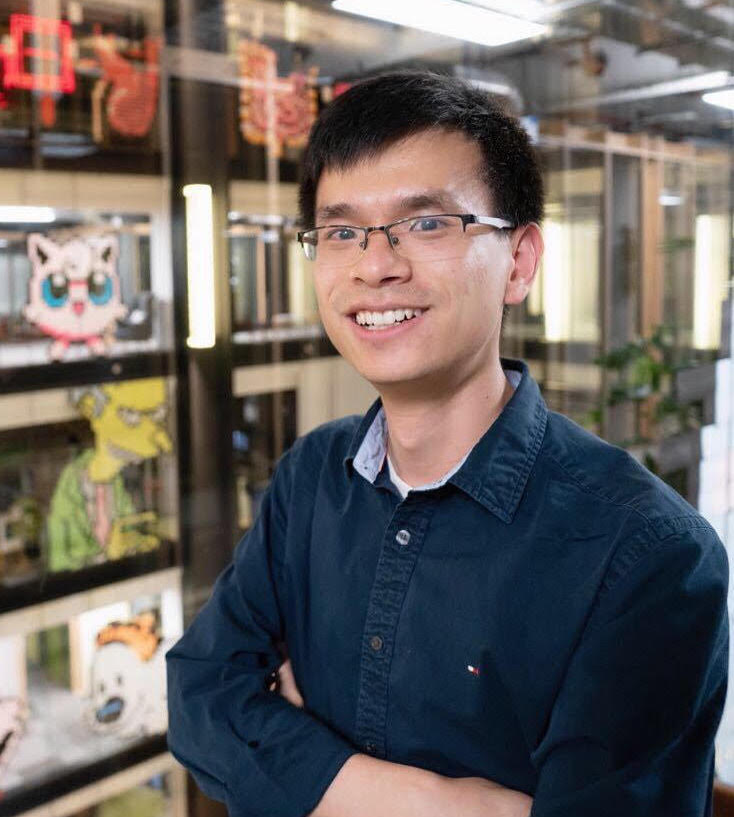
\includegraphics[width=0.2\textwidth]{organizers/xujie}
        \end{wrapfigure}
        \textbf{Xujie Si} is an Assistant Professor and Canada CIFAR AI Chair in the School of Computer Science at McGill University and at Mila - Quebec AI Institute. He finished his Ph.D. in Computer and Information Science at the University of Pennsylvania in 2020, advised by Prof. Mayur Naik. Xujie received my M.S. in computer science from Vanderbilt University in 2014, before which he obtained his B.E. (with Honors) from Nankai Unversity in 2011. He spent the summer of 2019 as a research scientist intern at DeepMind working with Pushmeet Kohli in the Robust AI team.\\
        \faHome: \url{https://www.cs.mcgill.ca/~xsi/} \faTwitter: \href{https://twitter.com/xujiesi}{@XujieSi}
    \end{figure}

    \begin{figure}[H]
        \begin{wrapfigure}{l}{0.2\textwidth}
            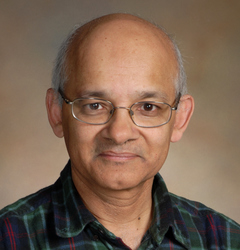
\includegraphics[width=0.2\textwidth]{organizers/prakash}
        \end{wrapfigure}
        \textbf{Prakash Panangaden} is a Professor at McGill University. He has three research areas: (a) semantics and logics for probabilistic systems and languages (b) machine learning and (c) quantum information theory. His research studies the approximation of continuous-state systems and associated metrics and logics. He is working on a quantitative extension of equational logic which allows one to carry out approximate reasoning equationally. Prakash is also interested in duality for automata and using it for minimization and recently has begun working on diffusion and similar continuous-time Markov processes.\\
        \faHome: \url{https://www.cs.mcgill.ca/~prakash/} \faTwitter: \href{https://twitter.com/prakash127}{@prakash127}
    \end{figure}
\end{document}